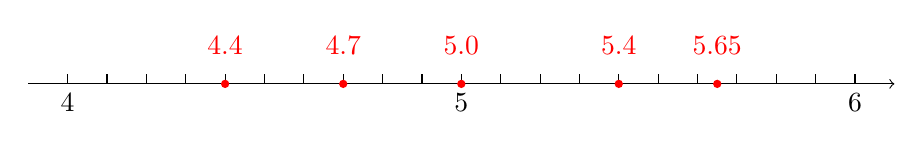
\begin{tikzpicture}[x=5cm]\draw[->](3.9,0)--(6.1,0);\foreach\i in{0,...,20}{\pgfmathsetmacro{\x}{4+\i/10}\draw(\x,0)--(\x,.12);}\foreach\x in{4,5,6}\node[below]at(\x,0){\x};\foreach\x/\t in{4.4/4.4,4.7/4.7,5/5.0,5.4/5.4,5.65/5.65}\fill[red](\x,0)circle(1.5pt)node[above=7pt]{\t};\end{tikzpicture}
